\documentclass[a4paper, 12pt]{article}

\usepackage[top=2cm, bottom=2cm, left=2.5cm, right=2.5cm]{geometry}
\usepackage[utf8]{inputenc}
\usepackage{amsmath, amsfonts, amssymb}
\usepackage{graphicx} % inserir figuras - \includegraphics[scale=•]{•}
\usepackage{float} % ignorar regras de tipografia e inserir figura aonde queremos.
\usepackage[brazil]{babel} % Trocar Figure para Figura.
\usepackage{indentfirst}
\pagestyle{empty}


\begin{document}
\begin{figure}[H]
	
\includegraphics[scale=0.9]{UnB_CiC_Logo.jpg}
\end{figure}
\noindent\rule{\textwidth}{0.4pt}
\begin{center}
	\textbf{{\Large Introdução à Ciência da Computação - 113913}} \newline \newline
	\textbf{{\large Lista de Exercícios 2} \\
	\vspace{9pt}
	{\large Condicionais}} \\
	\noindent\rule{\textwidth}{0.4pt}
	\newline
\end{center}

\textbf{{\large Observações:}}
\begin{itemize}
	\item As listas de exercícios serão corrigidas por um corretor automático, portanto é necessário que as entradas e saídas do seu programa estejam conforme o padrão especificado em cada questão (exemplo de entrada e saída). Por exemplo, não use mensagens escritas durante o desenvolvimento do seu código como “Informe a primeira entrada”. Estas mensagens não são tratadas pelo corretor, portanto a correção irá resultar em resposta errada, mesmo que seu código esteja correto.
	\item As questões estão em ordem de dificuldade. Cada lista possui 7 exercícios, sendo 1 questão fácil, 3 ou 4 médias e 2 ou 3 difíceis.
	\item Assim como as listas, as provas devem ser feitas na versão Python 3 ou superior.
	\item Leia com atenção e faça exatamente o que está sendo pedido.
\end{itemize}
\newpage % Questão A 
\begin{center}
\textbf{{\Large Questão A - Pares e Ímpares}}
\end{center}
\vspace{5pt}
Faça um programa que imprima na tela se um número lido do teclado é par ou ímpar. Se for par imprima também o próximo número par, caso contrário imprima o próximo ímpar.
\newline \newline
\textbf{{\large Entrada}} \newline
Apenas um inteiro.
\newline \newline
\textbf{{\large Saída}} \newline
A saída conterá duas linhas, uma informando se o número é par ou ímpar e outra mostrando o próximo par ou ímpar, conforme exemplo abaixo.
\newline
\begin{table}[H]
	\centering
	\begin{tabular}{|l|l|}
	\hline
	\textbf{Exemplo de Entrada} & \textbf{Exemplo de Saída} \\ \hline
	2 & 
	\begin{tabular}{l}
	2 é par \\
	4
	\end{tabular} \\ \hline
	
	3 & 	
	\begin{tabular}{l}
	3 é ímpar \\
	5
	\end{tabular} \\ \hline
	
	-4 & 
	\begin{tabular}{l}
	-4 é par \\
	-2
	\end{tabular} \\ \hline
	
	\end{tabular}
	\caption{Questão A}
	\label{tabela1}
\end{table}

\newpage % Questão B
\begin{center}
\textbf{{\Large Questão B - Índice de Massa Corporal}}
\end{center}
\vspace{5pt}
Usando como dados de entrada altura \textbf{\textit{h}} (em metros) e peso \textit{\textbf{p}} (em quilos), elabore um programa que calcule o IMC (índice de massa corporal) do usuário, usando a fórmula:
$$ \textrm{IMC} = \dfrac{p}{h^2} $$
Depois interprete e informe o resultado, da seguinte forma: 
\begin{itemize}
	\item \textbf{Baixo peso}: IMC abaixo de 18,5 $kg/m^2$
	\item \textbf{Peso normal}: IMC entre 18,5 e 24,9 $kg/m^2$
	\item \textbf{Sobrepeso}: IMC entre 24,9 e 29,9 $kg/m^2$
	\item \textbf{Obesidade Grau I}: IMC entre 29,9 e 34,9 $kg/m^2$
	\item \textbf{Obesidade Grau II}: IMC entre 34,9 e 39,9 $kg/m^2$
	\item \textbf{Obesidade Grau III}: IMC maior que 39,9 $kg/m^2$
\end{itemize}
Caso ele esteja acima da faixa de peso normal informe também o mínimo de quilos que serão necessários perder para chegar à faixa peso normal. 
\newline \newline
\textbf{{\large Entrada}} \newline
Duas linhas de dados: peso (em kg) e altura (em metros).
\newline \newline
\textbf{{\large Saída}} \newline
Caso o usuário esteja na faixa Baixo peso ou Peso normal apenas imprima a mensagem informando o IMC e, na próxima linha, a sua classificação correspondente usando a tabela, conforme exemplo fornecido abaixo. Caso contrário, imprima também o peso \textbf{mínimo} necessário a se perder para chegar à faixa peso normal com 2 casas decimais após a vírgula.
\newline
\begin{table}[H]
	\centering
	\begin{tabular}{|l|l|}
	\hline
	\textbf{Exemplo de Entrada} & \textbf{Exemplo de Saída} \\ \hline
	\begin{tabular}{l}
	79 \\
	1.84
	\end{tabular} & 
	\begin{tabular}{l}
	23.33 \\
	Peso normal
	\end{tabular} \\ \hline
	
	\begin{tabular}{l}
	84.4 \\
	1.85
	\end{tabular} & 
	\begin{tabular}{l}
	24.66 \\
	Peso normal
	\end{tabular} \\ \hline
	
	\begin{tabular}{l}
	85 \\
	1.60
	\end{tabular} & 
	\begin{tabular}{l}
	33.20 \\
	Obesidade grau I \\
	21.26
	\end{tabular} \\ \hline
	\end{tabular}
	\caption{Questão B}
	\label{tabela2}
\end{table}

\newpage % Questão C
\begin{center}
\textbf{{\Large Questão C - Tipos de Triângulos}}
\end{center}
\vspace{5pt}
Leia 3 valores de ponto flutuante A, B e C e ordene-os de modo que A representa o maior dos 3 lados. A seguir, determine o tipo de triângulo que estes três lados formam, com base nos seguintes casos, sempre escrevendo uma mensagem adequada:
\begin{itemize}
	\item Se $A \geq B + C$, apresente a mensagem: \textbf{NAO FORMA TRIANGULO}
	\item Se $A^2 = B^2 + C^2$, apresente a mensagem: \textbf{TRIANGULO RETANGULO}
	\item Se os três lados forem iguais, apresente a mensagem: \textbf{TRIANGULO EQUILATERO}
	\item Se apenas dois dos lados forem iguais, apresente a mensagem: \textbf{TRIANGULO ISOSCELES}
	\item Caso contrário, apresente a mensagem: \textbf{TRIANGULO ACUTANGULO OU OBTUSANGULO}
\end{itemize}
\textbf{{\large Entrada}} \newline
A entrada contém 3 valores reais todos maiores que zero. Não terá como entrada um valor tal que o triângulo seja retângulo e isósceles ao mesmo tempo.
\newline \newline
\textbf{{\large Saída}} \newline
Imprima a classificação do triângulo.
\newline
\begin{table}[H]
	\centering
	\begin{tabular}{|l|l|}
	\hline
	\textbf{Exemplo de Entrada} & \textbf{Exemplo de Saída} \\ \hline
	\begin{tabular}{l}
	7.0 \\
	5.0 \\
	7.0 
	\end{tabular} & TRIANGULO ISOSCELES \\ \hline
	
	\begin{tabular}{l}
	6.0 \\
	6.0 \\
	6.0 
	\end{tabular} & TRIANGULO EQUILATERO \\ \hline
	
	\begin{tabular}{l}
	1.0 \\
	3.0 \\
	1.0 
	\end{tabular} & NAO FORMA TRIANGULO \\ \hline
	\end{tabular}
	\caption{Questão C}
	\label{tabela3}
\end{table}

\newpage % Questão D
\begin{center}
\textbf{{\Large Questão D - Ghost e a Escada}}
\end{center}
\vspace{5pt}
No caminho para encontrar Jon Snow em Dragonstone, o lobo Ghost enfrenta um problema, uma grande escada. As escadas são numeradas de 1 até infinito. Sendo um lobo esperto, Ghost decidiu calcular dois valores, o número de escadas percorridas com números pares e ímpares. \newline \newline
Você precisa checar se o número de passos em escadas pares e ímpares encontrados pelo Ghost estão corretos. Considere que ele não pula nenhuma escada e que ele sobe, pelo menos, a escada de número 1. 
\newline \newline
\textbf{{\large Entrada}} \newline
Em uma única linha são dados dois inteiros \textit{\textbf{a, b}} $(0 \leq \textrm{a,b} \leq 100)$, o número de passos pares e ímpares, respectivamente. 
\newline \newline
\textbf{{\large Saída}} \newline
Em uma única linha, imprima ``a b ok'', se Ghost calculou corretamente os valores e ``a b errados'' caso contrário.
\newline \newline
\textbf{{\large Nota}} \newline
Lembre-se que para ler vários valores em uma mesma linha, use \textbf{\textit{input().split()}}. Se o argumento de split for vazio, o separador das variáveis é um espaço em branco. Porém, \textbf{input lê apenas strings do teclado}, portanto você deverá converter as strings em floats. No exemplo a seguir, o usuário digita valores separados por um espaço em branco e aperta enter para enviá-los, então, o programa lê esses valores separados por espaços como strings (na ordem em que aparecem), guardados nas variáveis correspondentes e os converte para inteiros: \newline
\textbf{\textit{A, B = input().split() \newline
A, B = [int(A), int(B)]}}
\newline
\begin{table}[H]
	\centering
	\begin{tabular}{|l|l|}
	\hline
	\textbf{Exemplo de Entrada} & \textbf{Exemplo de Saída} \\ \hline
	2 3 & 2 3 ok \\ \hline
	3 1 & 3 1 errados \\ \hline
	5 5 & 5 5 ok \\ \hline
	\end{tabular}
	\caption{Questão D}
	\label{tabela4}
\end{table}

\newpage % Questão E
\begin{center}
\textbf{{\Large Questão E - Calendário}}
\end{center}
\vspace{5pt}
Raphael quer fazer um calendário para o mês atual. Para isso, ele desenha um tabela aonde as colunas correspondem às semanas (uma semana são 7 dias consecutivos de Segunda até Domingo), linhas correspondem aos dias da semana, e as células contém datas. Por exemplo, o calendário para Janeiro de 2017 seria como na imagem abaixo:
\begin{figure}[H]
	\centering
	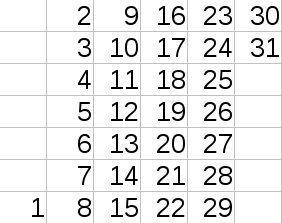
\includegraphics[scale=0.9]{Calendario.png} 
\end{figure} 
Raphael quer saber quantas colunas sua tabela deve ter, dado o mês e o dia da semana do primeiro dia do mês. Você pode fazer um programa para ajudá-lo, assumindo que o ano não é bissexto?
\newline \newline
\textbf{{\large Entrada}} \newline
A entrada consiste de uma única linha contendo dois inteiros \textbf{\textit{m}} e \textbf{\textit{d}} 
$(1 \leq \textrm{m} \leq 12\textrm{,} \, 1 \leq \textrm{d} \leq 7)$, o número do mês e o dia da semana do primeiro dia do mês (1 é Segunda, 7 é Domingo).
\newline \newline
\textbf{{\large Saída}} \newline
Imprima um único inteiro: o número de colunas que a tabela terá. O primeiro exemplo corresponde a Janeiro de 2017, mostrado na figura acima. 
\newline
\begin{table}[H]
	\centering
	\begin{tabular}{|l|l|}
	\hline
	\textbf{Exemplo de Entrada} & \textbf{Exemplo de Saída} \\ \hline
	1 7 & 6 \\ \hline
	1 1 & 5 \\ \hline
	11 6 & 5 \\ \hline
	\end{tabular}
	\caption{Questão E}
	\label{tabela5}
\end{table}

\newpage % Questão F
\begin{center}
\textbf{{\Large Questão F - O Jogo}}
\end{center}
\vspace{5pt}
Leia a hora inicial, minuto inicial, hora final e minuto final de um jogo. A seguir calcule a duração do jogo, considerando que o jogo pode acabar em um dia e terminar em outro, tendo uma duração máxima de 24 horas.
\newline \newline
\textbf{{\large Entrada}} \newline
Quatro números inteiros representando a hora de início e fim do jogo.
\newline \newline
\textbf{{\large Saída}} \newline
Mostre a seguinte mensagem: ``O jogo durou XX hora(s) e YY minuto(s).''
\newline
\begin{table}[H]
	\centering
	\begin{tabular}{|l|l|}
	\hline
	\textbf{Exemplo de Entrada} & \textbf{Exemplo de Saída} \\ \hline
	7 5 7 4 & O jogo durou 23 hora(s) e 59 minuto(s). \\ \hline
	7 7 7 7 & O jogo durou 24 hora(s) e 0 minuto(s). \\ \hline
	7 10 8 9 & O jogo durou 0 hora(s) e 59 minuto(s). \\ \hline
	\end{tabular}
	\caption{Questão F}
	\label{tabela6}
\end{table}

\newpage % Questão G
\begin{center}
\textbf{{\Large Questão G - A mais Longa Subsequência Incomum}}
\end{center}
\vspace{5pt}
Uma subsequência de uma string é uma sequência de caracteres que aparece na mesma ordem da string. As ocorrências não precisam ser consecutivas, por exemplo, ``\textit{ac}'', ``\textit{bc}'', ``\textit{abc}'' e ``\textit{a}'' são subsequências da string ``\textit{abc}'', enquanto as strings ``\textit{abbc}'' e
``\textit{acb}'' não são. A string vazia é subsequência de qualquer string. Qualquer string é subsequência dela mesmo. \newline \newline
Dada duas strings \textbf{\textit{a}} e \textbf{\textit{b}}, encontre o tamanho da maior subsequência incomum, que é a maior string que é subsequência de uma das duas e não é subsequência da outra.
\newline \newline
\textbf{{\large Entrada}} \newline
A primeira linha contém a string \textbf{\textit{a}} e a segunda linha contém a string \textbf{\textit{b}}. As duas strings não são vazias e são compostas apenas por letras minúsculas.
\newline \newline
\textbf{{\large Saída}} \newline
Se não houver nenhuma subsequência incomum, imprima ``-1''. Caso contrário imprima o tamanho da maior subsequência incomum de \textbf{\textit{a}} e \textbf{\textit{b}}.
\newline \newline
\textbf{{\large Dica}} \newline
Existe uma função em Python que retorna o tamanho de uma string qualquer dada como parâmetro.
\newline \newline
\textbf{{\large Nota}} \newline
No primeiro exemplo você pode escolher ``defgh'' da string b como a maior subsequência da string que não aparece como subsequência da string a.
\newline
\begin{table}[H]
	\centering
	\begin{tabular}{|l|l|}
	\hline
	\textbf{Exemplo de Entrada} & \textbf{Exemplo de Saída} \\ \hline
	\begin{tabular}{l}
	abcd \\
	defgh
	\end{tabular} & 5 \\ \hline
	
	\begin{tabular}{l}
	a \\
	a
	\end{tabular} & -1 \\ \hline
	
	\begin{tabular}{l}
	aaaaaaaaaacccccccccc \\
	aaaaaaaaaadddddddddd
	\end{tabular} & 20 \\ \hline
	\end{tabular}
	\caption{Questão G}
	\label{tabela7}
\end{table}
\end{document}